\subsection{Estimated Parameters}
\label{subsec:estimated_params}


\FloatBarrier

We estimate parameters that cannot be calibrated outside of the model with the method of
simulated moments \citep{McFadden1989} by minimizing the distance between simulated and
observed infection rates (disaggregated by region and age groups) and fatality rates.
Since our model includes a lot of randomness, we average simulated infection rates over
several model runs.

All estimated parameters are described in Table~\ref{tab:estimated_params}.

\begin{landscape}

\begin{table}[htb]
    \centering
    \caption{Estimated Parameters}
    \label{tab:estimated_params}
    \input{../bld/param_tables/estimates}
\end{table}

\end{landscape}


We fit our model to data for Germany from mid September 2020 until June 2021. We do not
use earlier periods for three reasons. Firstly, in the beginning PCR tests were very
scarce and the reported case numbers unreliable. Secondly, during the summer the case
numbers were extremely low. This could lead to the epidemic going extinct in our
simulation. Thirdly, over the summer, imported cases from touristic travel were likely
important for the infection dynamic but there is not enough data to include them into our
model.

% infection probabilities
To avoid over-fitting and simplify the numerical optimization problem, we only allow for
five different infection probabilities: 1) for contacts in schools 2) for contacts in
preschools and nurseries. 3) for work contacts. 4) for households. 5) for other
contacts.

Since the infectiousness of a contact between an infectious and a susceptible
person depends on many things, the numerical values of the infection probabilities in
Table~\ref{tab:estimated_params} only reflect a base probability. This
base probability is modified by a seasonality factor, an age specific
susceptiblity factor and an infectiousness factor that depends on the virus strand
of the infected person. The base infection probability is only equal to the actual
infection probability when all of those factors are 1. This would be the
case for a contact between an 80+ year old susceptible person with a person who is
infected with the B.1.1.7 strand of the virus on January first.

It is not possible to rank different types of contacts according to their
infectiousness just from the numerical values of the infection probabilities.
There are two reasons for this: Firstly, for computational reasons the
seasonality factor is normalized such that it reaches 1 at its peak. It has thus
a lower average for contact types with strong seasonality (e.g. other contacts) than for
contact types with weak seasonality (e.g. work contacts). Secondly, for household and
school contacts we do not have data on whether people actually have physical contact.
Thus the infection probabilities for those contact types are actually the product of the
probability to actually have physical contact on a given day and the infection
probability of that contact.

In order to get a feeling for the infectiousness of each contact type it
is more intuitive to look at how many infections were actually caused by each contact
type. This is depicted in Figure~\ref{fig:infection_heatmap}. We can see that work and
other contacts are the main drivers of the pandemic, followed by infections in
households. Schools and preschools contribute fewer infections which is to be expected
given that there are much fewer students than working adults in the German population.
Nevertheless, Figure~\ref{fig:school_scenarios_detailed} shows that schools do have a
notable effect on the infection dynamic in the long run.

\begin{figure}
    \centering
    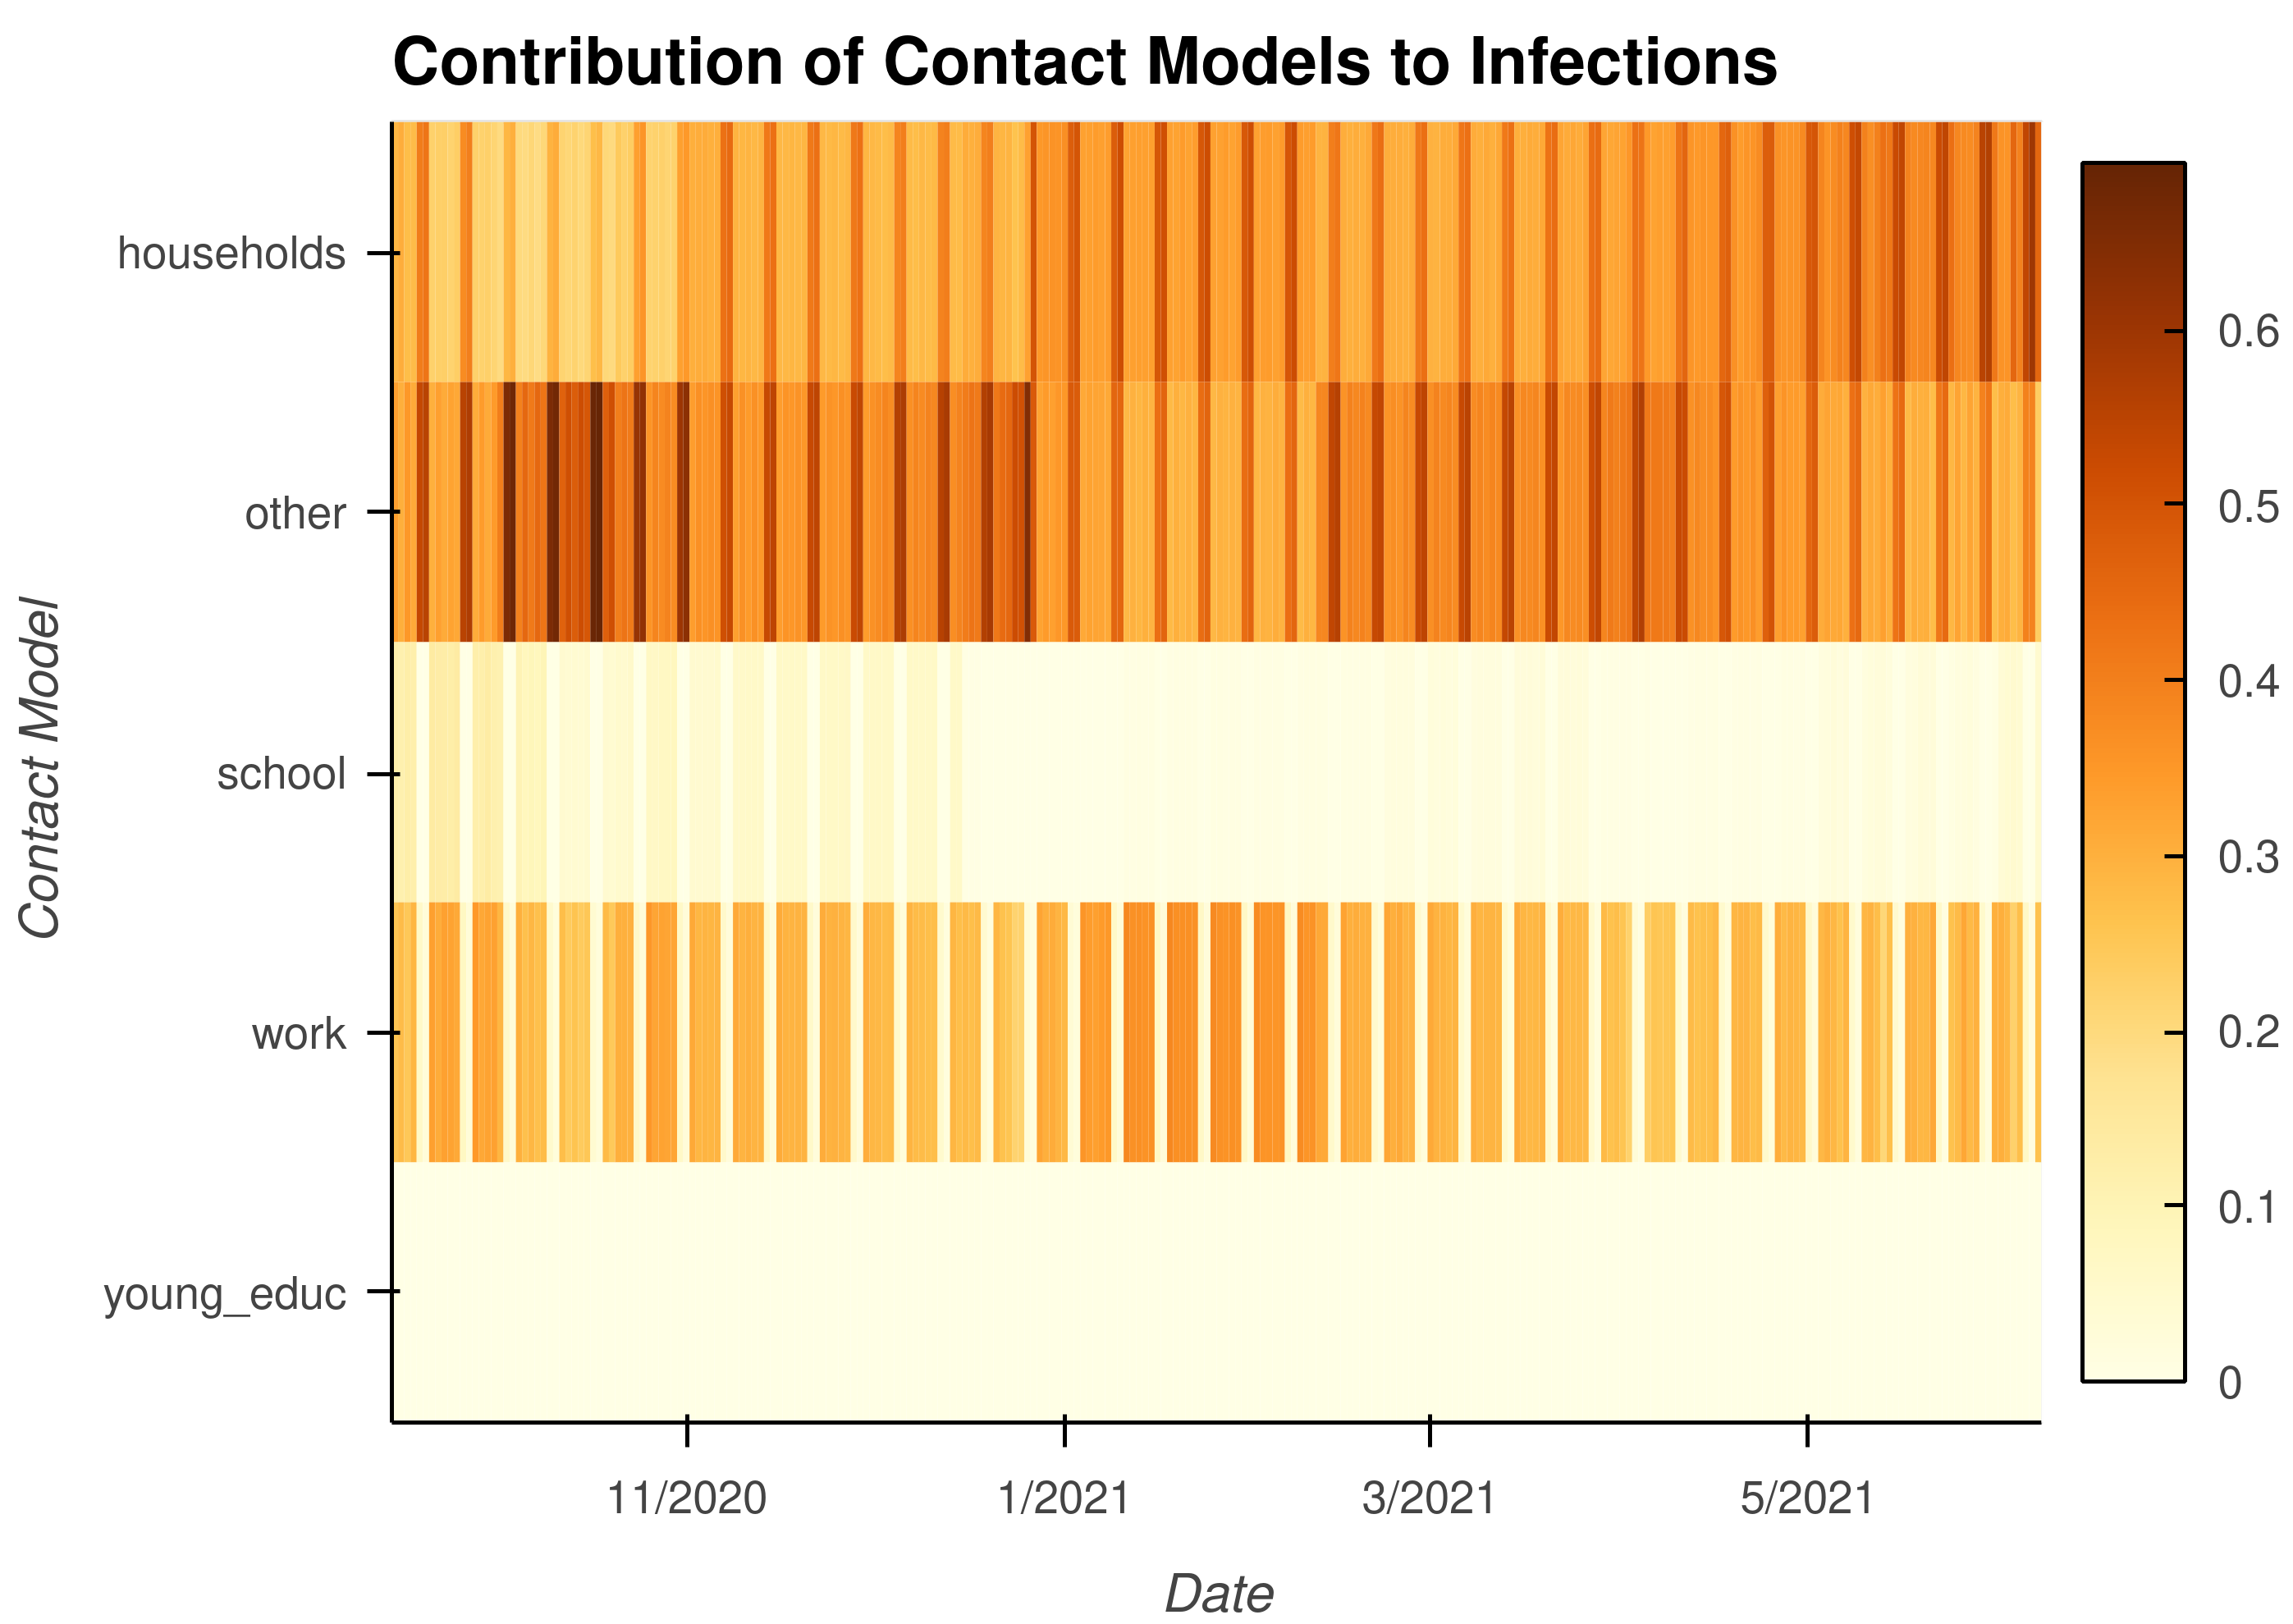
\includegraphics[width=\textwidth]{figures/infection_channels.png}
    \caption{Daily share of infections by contact type}
    \floatfoot{\noindent \textit{Note:} Daily share of infections that were contributed
    by each contact type. Darker colors mean that a larger share of infections were
    contributed by that contact type. The majority of infections take place in the
    workplace, in households and via other contacts. Schools and preschools contribute
    less infections, especially after hygiene measures have been introduced.}
    \label{fig:infection_heatmap}
\end{figure}

We also estimate a parameter that reflects the effect of hygiene measures
at work and in educational facilities. This parameter becomes active in November 2020
when stricter mask mandates and distancing rules were introduced. It is estimated to
reduce infectiousness of contacts by one third.

Moreover, we estimate nine different multipliers that reflect how strongly other contacts
are reduced over time. The dates at which we switch between the multipliers usually
coincide with policy changes and is not determined from the \replaced[id=K]{case
numbers}{data}. The only exception to this are slight adjustments to parameters to
incorporate lockdown fatigue (towards the end of a lockdown period) or precautionary
contact reductions (in times of high incidences right before a lockdown is enacted). The
estimated other multipliers are also depicted in Figure~\ref{fig:other_multiplier}.

\begin{figure}
    \centering
    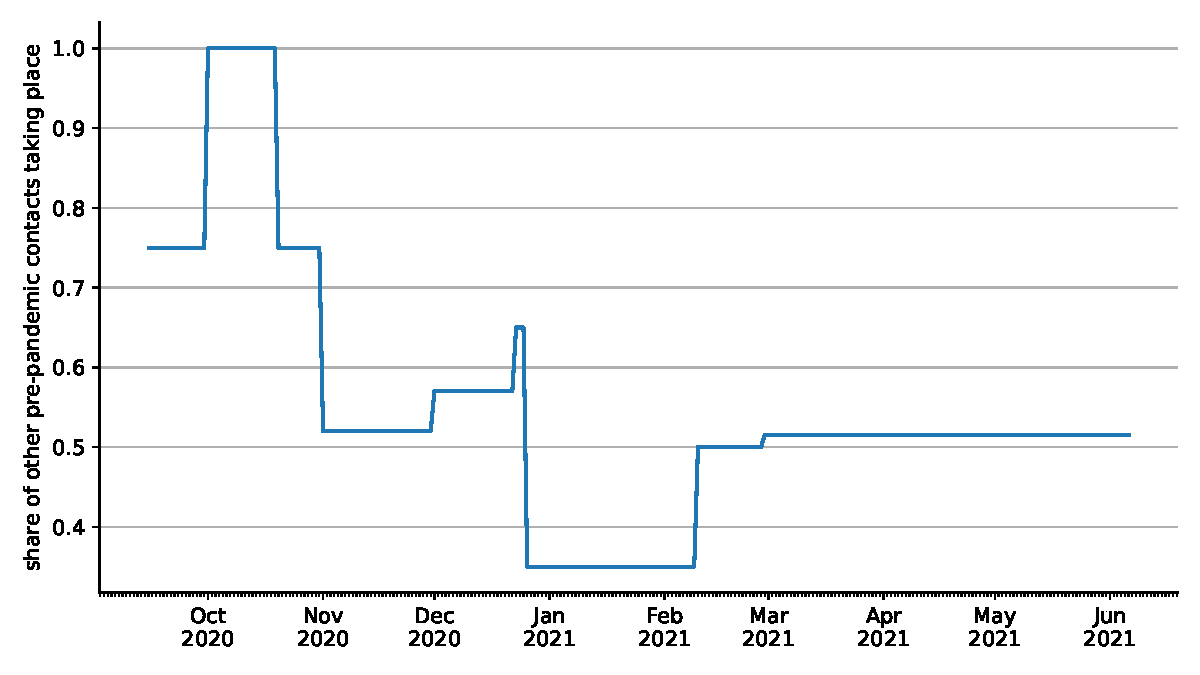
\includegraphics[width=0.5\textwidth]{figures/results/figures/data/other_multiplier}
    \caption{Share of Pre-Pandemic Other Contacts Taking Place with Infection Potential}
    \label{fig:other_multiplier}
    \floatfoot{\noindent \textit{Note:} Values of the other multiplier. All values are
    estimated via the method of simulated moments. The rationale behind each switching
    point is described in Table~\ref{tab:estimated_params}}
\end{figure}

While we estimate 9 different values for the other contact multiplier, they are not
estimated completely freely. In particular we ensure that the ordering of the parameter
values is consistent with the stringency of policies. For example, the strongest
contact reduction was estimated for January 2021 during where very strict measures
and curfews were in place, whereas the weakest contact reduction was in October 2020
where policies were very lenient.

Since we do not have good data on the reduction of other contacts, it is not possible
to separately estimate parameters for contact reduction and the effect of hygiene
measures. The reported other multipliers in Table~\ref{tab:estimated_params} are thus
a combination of contact reduction and hygiene measures.

Finally we estimate one parameter that governs the introduction of the B.1.1.7 virus
variant in January 2021. This parameter implies that at the end of January roughly one
case per 100 000 individuals per day is imported. After January we do not model imported
cases of B.1.1.7 anymore because they are negligible compared to the endogenous growth
of that virus variant.

While a formal identification argument is beyond the scope of this paper, below we give
a rough intuition which features of the data help us to estimate each parameter.

The different infection probabilities can be separately identified because the degree to
which each contact type is active varies over time (e.g. school closures, vacations and
different work from home policies) and they affect different subgroups of the population
differently (e.g. $\beta_{school}$ most strongly affects kids whereas
$\beta_{work}$ has the strongest effect on adults in working age and $\beta_{other}$
affects all age groups equally).
The hygiene and other multipliers can be identified because they are only active in
certain time periods. However, it is necessary to normalize one other multiplier to
1 because there is no period without any contact reduction in our data.
The introduction parameter for the B.1.1.7 mutation can be identified from the share of
that virus strand in the population. The rapid test
demand parameters are identified because rapid tests first lead to a very steep increase
in observed cases and then to a sudden decrease -- in a time where almost all other
things in the model would not cause a change in trend.